\section{Extracción de características}\label{sec:features}

\begin{frame}
    \frametitle{Extracción de características}

    \begin{block}{Sonido}
        Variación en la presión que ejerce el medio que lo transmite sobre su receptor.
        \begin{itemize}
            \item<2-> \textbf{Frecuencia}: Cantidad de vibraciones por segundo (medida en Hertz).
            \item<3-> \textbf{Amplitud}: Intensidad de las vibraciones (medida arbitraria).
        \end{itemize}
    \end{block}

    \begin{itemize}
        \item<4-> \textit{Periódicos}.
        \begin{itemize}
            \item Período (en segundos)
            \item Frecuencia (en Hertz)
        \end{itemize}
        \item<5-> \textit{Armónicos}.
        \item<6-> \textit{Ruidos}.
    \end{itemize}
\end{frame}

\begin{frame}
    \frametitle{Extracción de características}

    \begin{columns}
        \column{0.5\textwidth}

        \begin{figure}[!h]
            \centering
            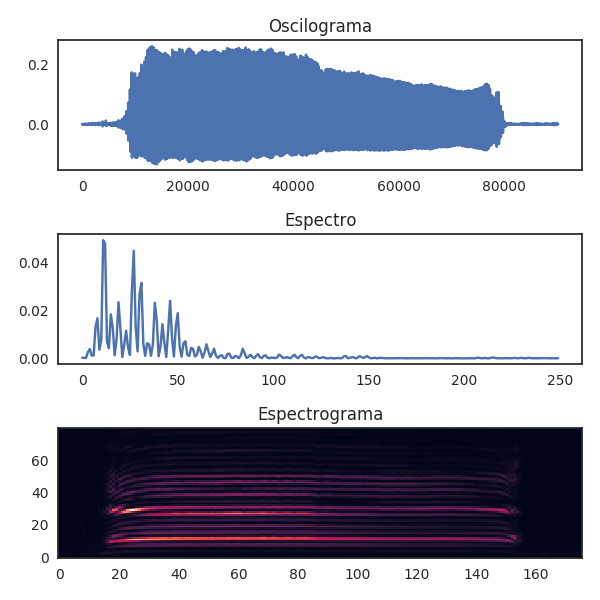
\includegraphics[width=\textwidth]{oscillogram+spectrum+spectrogram.png}
        \end{figure}

        \pause
        \column{0.5\textwidth}

        Pasos para la conversión de una señal del dominio analógico al digital:
        \begin{enumerate}
            \item<3-> \textbf{Filtrado} al intervalo de frecuencias $[0,B]$.
            \item<4-> \textbf{Muestreo} con frecuencia $F_s = 2B$.
            \item<5-> \textbf{Cuantificación}.
        \end{enumerate}

    \end{columns}
\end{frame}

\begin{frame}
    \frametitle{Tramas}

    \begin{itemize}
        \item $N$: Cantidad de muestras de la señal que contiene una trama.
        \item $M$: Cantidad de muestras diferentes en dos tramas consecutivas.
    \end{itemize}

    \pause
    \begin{block}{Obtención de la trama que comienza en la muestra $m$}
        \begin{equation*}
            s[n]_m = \begin{cases}
                         s[n + m]w(n) & 0\leq n\leq N-1 \\
                         0 & \text{eoc.}
            \end{cases}
        \end{equation*}
    \end{block}

    $w(n)$ \textit{función de ventana}. La más simple es $w(n)=1$.

    \pause
    \alert{\textit{Hanning}: $w(n) = 0.50 - 0.50 \cdot \cos \left( \frac{2\pi n}{N-1} \right)$}
\end{frame}

\begin{frame}
    \frametitle{Características temporales}

    \begin{columns}
        \column{0.5\textwidth}

        \begin{figure}[!h]
            \centering
            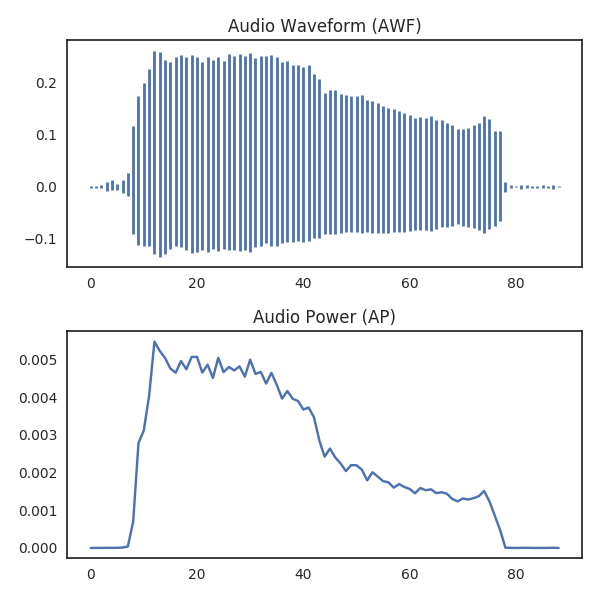
\includegraphics[width=\textwidth]{temporal-features-vertical.png}
        \end{figure}

        \column{0.5\textwidth}

        \begin{itemize}
            \item<2-> \textbf{Audio Waveform}: Vector de pares con el máximo y mínimo valor presentes en tramas no superpuestas ($N=M$).
            \item<3-> \textbf{Audio Power}: $AP = \frac{1}{N}\sum_{n=0}^{N-1}{|x[n]|^2}$
        \end{itemize}

    \end{columns}
\end{frame}

\begin{frame}
    \frametitle{Características temporales}

    \begin{itemize}
        \item<1-> \textbf{Log-Attack Time}: $LAT = \log_{10}{(stopAttack - startAttack)}$
        \item<2-> \textbf{Temporal Centroid}: $TC = \frac{\sum_{t=0}^{T-1}{AP_t \cdot t}}{\sum_{t=0}^{T-1}{AP_t}}$
        \item<3-> \textbf{Effective Duration}: Duración del intervalo de tiempo en que la señal es perceptible.
        \item<4-> \textbf{Auto-correlation}: $AC_k = \frac{1}{x[0]^2}\sum_{n=0}^{N-k-1}{x[n]\cdot x[n+k]}$
    \end{itemize}

\end{frame}

\begin{frame}
    \frametitle{Características espectrales}

    \begin{columns}
        \column{0.5\textwidth}

        \begin{block}{Transformada Discreta de Fourier}
            \begin{equation*}
                X[f] = \sum_{n=0}^{N-1}{x[n]e^{\frac{-i2\pi fn}{N}}}
            \end{equation*}
        \end{block}

        \column{0.5\textwidth}

        \begin{block}{Transformada Discreta Inversa}
            \begin{equation*}
                x[n] = \frac{1}{N}\sum_{f=0}^{N-1}{X[f]e^{\frac{i2\pi fn}{N}}}
            \end{equation*}
        \end{block}
    \end{columns}

    \begin{itemize}
        \item<2-> Suelen considerarse solamente los últimos $\lceil (N+1)/2 \rceil$ valores de $X[n]$.
        \item<3-> La posición $k$-ésima del vector $X[k]$ contiene la amplitud correspondiente a la frecuencia $k\cdot(F_s/N)$ en la señal.
    \end{itemize}

\end{frame}

\begin{frame}
    \frametitle{Características espectrales}

    \begin{columns}
        \column{0.5\textwidth}

        \begin{figure}[!h]
            \centering
            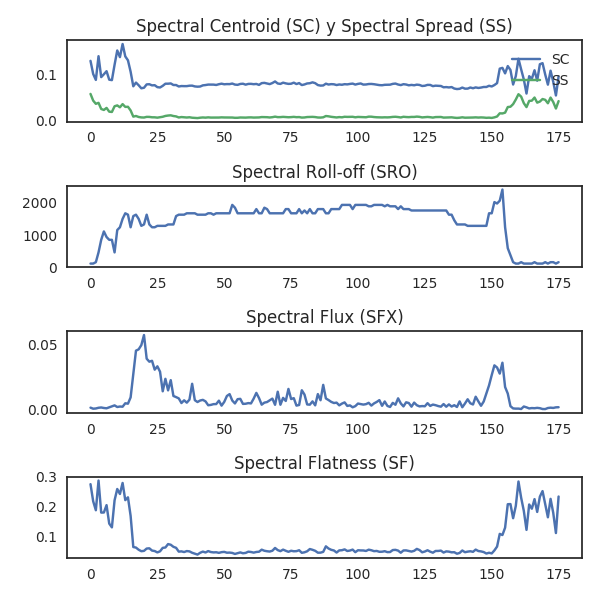
\includegraphics[width=\textwidth]{spectral-features-vertical.png}
        \end{figure}

        \column{0.5\textwidth}

        \begin{itemize}
            \item<2-> \textbf{Spectral Shape}:
            \begin{itemize}
                \item Spectral Centroid: Centro de masas del espectro
                \item Spectral Spread: Dispersión del espectro
                \item Spectral Roll-off: Frecuencia bajo la que se encuentra cierto porcentaje de la energía total
            \end{itemize}
            \item<3-> \textbf{Spectral Flux}
            \item<4-> \textbf{Spectral Flatness}
        \end{itemize}

    \end{columns}
\end{frame}

\begin{frame}
    \frametitle{Características armónicas}

    \begin{block}{Frecuencia Fundamental ($F_0$)}
        Es la frecuencia más baja del espectro de frecuencias tal que las frecuencias dominantes en la señal pueden expresarse como múltiplos de ella.
        Puede por tanto considerarse como la frecuencia de la señal armónica que mejor representa a la señal en cuestión.
    \end{block}

    \pause
    \begin{columns}
        \column{0.5\textwidth}

        {\tiny
        \begin{gather*}
            d_t'(\tau) = \begin{cases}
                             1 & \tau = 0 \\
                             \frac{d_t(\tau)}{\frac{1}{\tau}{\sum_{j=1}^{\tau}{d_t(j)}}} & eoc.
            \end{cases}\\
            d_t(\tau) = \sum_{i=0}^{N-1}{(x[i]-x[i+\tau])^2}
        \end{gather*}
        }

        \column{0.5\textwidth}

        \textbf{Algoritmo YIN}:\\
        $F_0$ es el valor $1/\tau$ tal que $\tau$ que minimiza la función $d_t'(\tau)$ para cada trama.

    \end{columns}
\end{frame}

\begin{frame}
    \frametitle{Características armónicas}

    \begin{block}{Picos armónicos}
        Se localizan en torno a los múltiplos de $F_0$.
        Se puede definir el $h$-ésimo pico armónico como el valor de la DFT de la señal localizado en la posición $k_h$ tal que:
        \begin{equation*}
            k_h = \argmax_{k\in [a_h,b_h]}|X[k]|
        \end{equation*}
    \end{block}

    donde los extremos del intervalo $[a_h, b_h]$ están dados por las ecuaciones:

    {\small
    \begin{columns}
        \column{0.5\textwidth}
        \begin{equation*}
            a_h = \text{floor}\left[ (h - nht)\frac{F_0}{\Delta F} \right]
        \end{equation*}

        \column{0.5\textwidth}
        \begin{equation*}
            b_h = \text{ceil}\left[ (h + nht)\frac{F_0}{\Delta F} \right]
        \end{equation*}
    \end{columns}
    }
\end{frame}

\begin{frame}
    \frametitle{Características armónicas}

    \begin{columns}
        \column{0.5\textwidth}

        \begin{figure}[!h]
            \centering
            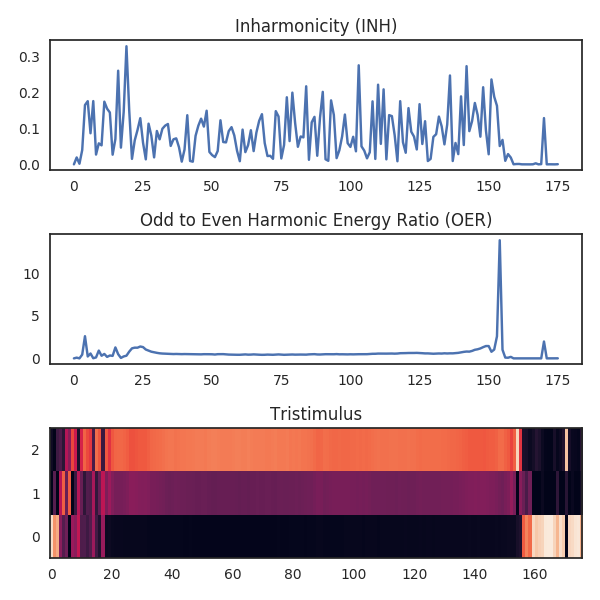
\includegraphics[width=\textwidth]{harmonic-features-vertical.png}
        \end{figure}

        \column{0.5\textwidth}

        \begin{itemize}
            \item<1-> \textbf{Inharmonicity}: Divergencia de las frecuencias que componen la señal respecto a los múltiplos de $F_0$.
            \item<2-> \textbf{Odd to Even Harmonic Energy Ratio}: Proporción entre múltiplos impares y pares de $F_0$.
            \item<3-> \textbf{Tristimulus}: Equivalente a los atributos de color en la visión.
        \end{itemize}

    \end{columns}
\end{frame}

\begin{frame}
    \frametitle{Mel Frequency Cepstral Coefficients}

    \begin{columns}
        \pause
        \column{0.5\textwidth}

        \begin{itemize}
            \item Caracterizar el contenido relevante de la señal, obviando características que aportan poca información.
            \begin{itemize}
                \item ruido de fondo
                \item emociones
                \item volumen
                \item tono
            \end{itemize}
            \item Desarrollada para el reconocimiento automático del habla humana.
        \end{itemize}

        \pause
        \column{0.5\textwidth}

        \begin{figure}[!h]
            \centering
            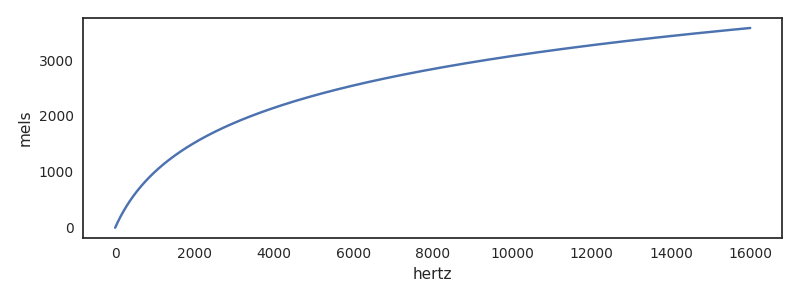
\includegraphics[width=\textwidth]{mel-scale-wide.png}
        \end{figure}

        \begin{block}{Escala Mel}
            \begin{equation*}
                m = 2595\log_{10}\left( 1 + \frac{f}{700} \right)
            \end{equation*}
        \end{block}

    \end{columns}
\end{frame}

\begin{frame}
    \frametitle{Mel Frequency Cepstral Coefficients}

    \begin{columns}
        \pause
        \column{0.5\textwidth}

        \begin{block}{Banco de filtros de Mel}
            \begin{itemize}
                \item Se divide el intervalo de frecuencias en M + 2 puntos.
                \item Se convierten a Mel.
            \end{itemize}
        \end{block}

        \pause
        \column{0.5\textwidth}

        {\small
        \begin{equation*}
            H_m(k) = \begin{cases}
                         0 & k < f_{m-1} \\
                         \frac{k-f_{m-1}}{f_m - f_{m-1}} & f_{m-1}\leq k\leq f_m \\
                         \frac{f_{m+1}-k}{f_{m+1}-f_m} & f_m \leq k\leq f_{m+1} \\
                         0 & k > f_{m+1} \\
            \end{cases}
        \end{equation*}
        }
    \end{columns}

    \pause

    \begin{figure}[!h]
        \centering
        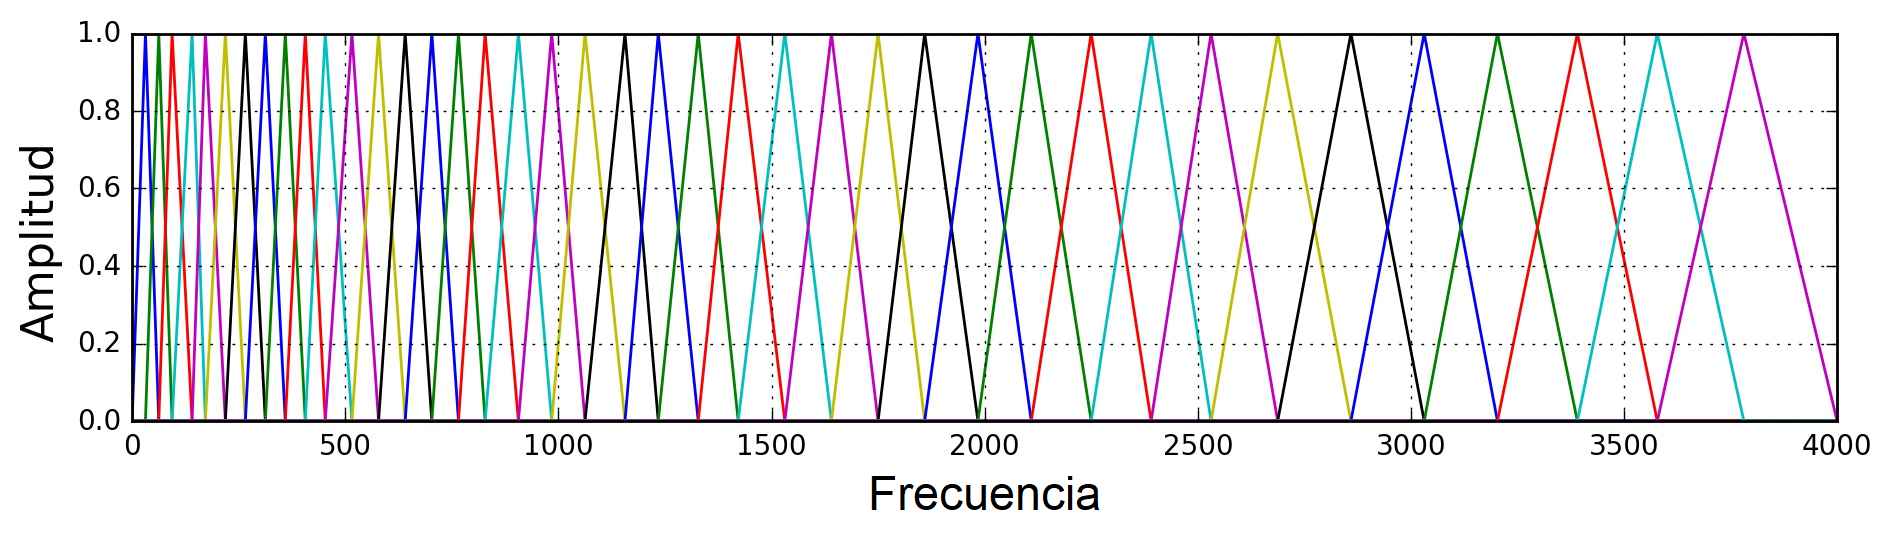
\includegraphics[width=0.8\textwidth]{mel-filters.png}
    \end{figure}
\end{frame}

\begin{frame}
    \frametitle{Mel Frequency Cepstral Coefficients}

    \begin{enumerate}
        \item<1-> Descomponer la señal $s[n]$ en tramas $s[n]_m = x[n]$.
        \item<2-> Por cada trama calcular la potencia espectral, cuya $k$-ésima componente se calcula por
        \begin{equation*}
            P[k] = \frac{|X[k]|^2}{K}
        \end{equation*}
        \item<3-> Aplicar el banco de filtros de Mel a $P[k]$ y sumar las energías de cada filtro.
        \item<4-> Calcular el logaritmo de las componentes (energías).
        \item<5-> Aplicar la transformada de coseno discreta (DCT) al vector de los logaritmos.
    \end{enumerate}
\end{frame}

\begin{frame}
    \frametitle{Mel Frequency Cepstral Coefficients}

    \begin{columns}
        \column{0.5\textwidth}

        \begin{block}{Transformada de Coseno Discreta}
        {\small
        \begin{equation*}
            f[j] = \sum_{m=0}^{M-1}{e[m]\cos{\left[ \frac{\pi}{M}j\left( m + \frac{1}{2} \right) \right]}}
        \end{equation*}
        }
        \end{block}

        \begin{block}{Deltas}
        {\small
        \begin{equation*}
            d_t = \frac{\sum_{n=1}^{T}{n(c_{t+n} - c_{t-n})}}{2\sum_{n=1}^{T}{n^2}}
        \end{equation*}
        }
        \end{block}

        \column{0.5\textwidth}

        \begin{figure}[!h]
            \centering
            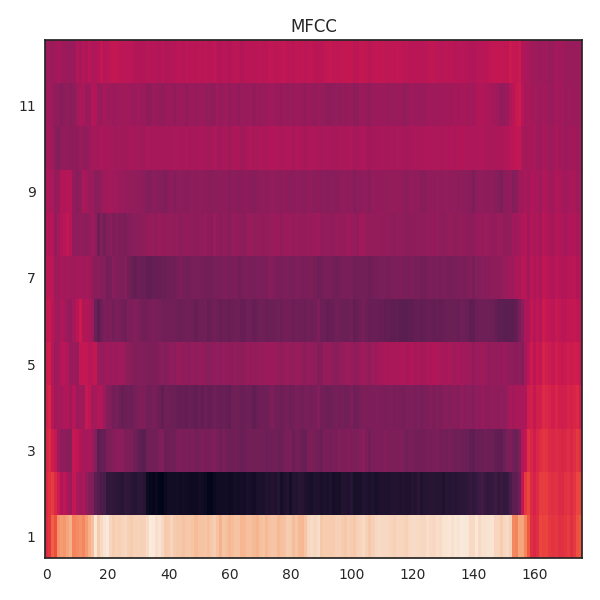
\includegraphics[width=\textwidth]{mfcc-square.png}
        \end{figure}

    \end{columns}
\end{frame}

